\documentclass[12pt,a4paper]{article}
\usepackage[UTF8]{ctex}
\usepackage{amsmath,amssymb}
\usepackage{listings}
\usepackage{xcolor}
\usepackage{hyperref}
\usepackage{geometry}
\usepackage{graphicx}
\geometry{margin=2.5cm}

\lstdefinestyle{python}{
  language=Python,
  basicstyle=\ttfamily\small,
  keywordstyle=\color{blue}\bfseries,
  commentstyle=\color{gray},
  stringstyle=\color{red},
  showstringspaces=false,
  breaklines=true,
  frame=single,
  backgroundcolor=\color{gray!10}
}

\title{Swap Test / Swap 测试}
\author{QuoNic}
\date{}

\begin{document}
\maketitle

\begin{center}
\textbf{Algorithms / 算法} | 难度：中级 | 预计时间：10 分钟
\end{center}

\tableofcontents
\newpage

\section{为什么需要？}

Swap 测试用于估计两个量子态的重叠度，是量子信息处理的基本工具。

\subsection{经典局限}
\b\begin{itemize}
  \item 经典方法需要多次测量才能估计重叠度
  \item 对于未知量子态，经典方法效率低
\end{itemize}

\subsection{量子优势}
\b\begin{itemize}
  \item Swap 测试只需要 1 个辅助量子比特
  \item 可以高效估计 $|\langle\psi|\phi\rangle|^2$
  \item 是量子机器学习的基础
\end{itemize}

\subsection{实际应用}
\b\begin{itemize}
  \item 量子态比较
  \item 量子机器学习（核方法）
  \item 量子通信（态验证）
\end{itemize}

\section{快速上手}

\begin{lstlisting}[style=python]
from quonic.algorithms import swap_test

# Compare two states
result = swap_test(state1="0", state2="0")
print(f"Overlap: {result.overlap:.3f}")
\end{lstlisting}

\textbf{预期输出}：
\begin{verbatim}
Overlap: 1.000
\end{verbatim}

\section{原理详解}

\subsection{电路图}

\begin{center}
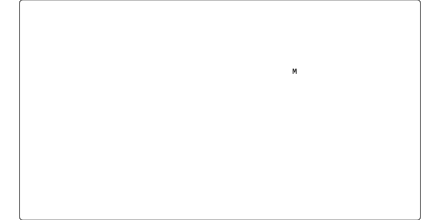
\includegraphics[width=0.6\textwidth]{../../images/swap_test_circuit.svg}
\end{center}

\subsection{数学推导}

Swap 测试估计两个量子态的重叠度：
\begin{equation}
P(|0\rangle) = \frac{1 + |\langle\psi|\phi\rangle|^2}{2}
\end{equation}

因此：
\begin{equation}
|\langle\psi|\phi\rangle|^2 = 2P(|0\rangle) - 1
\end{equation}

\subsection{几何解释}

Swap 测试通过受控 Swap 门和 Hadamard 门，将两个量子态的重叠度编码到辅助量子比特的测量概率中。

\section{代码详解}

\begin{lstlisting}[style=python]
from quonic.algorithms import swap_test

# swap_test(state1, state2, shots)
# state1, state2: quantum states to compare
# shots: number of measurements
result = swap_test(state1="0", state2="0", shots=1024)

# result.overlap: estimated overlap |<psi|phi>|^2
# result.prob_0: probability of measuring |0>
print(f"Overlap: {result.overlap:.3f}")
\end{lstlisting}

\section{进阶用法}

\subsection{场景 1：不同态}

\begin{lstlisting}[style=python]
# Compare orthogonal states
result = swap_test(state1="0", state2="1")
print(f"Overlap: {result.overlap:.3f}")  # ~0

# Compare identical states
result = swap_test(state1="+", state2="+")
print(f"Overlap: {result.overlap:.3f}")  # ~1
\end{lstlisting}

\subsection{场景 2：多量子比特态}

\begin{lstlisting}[style=python]
# Compare multi-qubit states
result = swap_test(state1="00", state2="11")
print(f"Overlap: {result.overlap:.3f}")
\end{lstlisting}

\section{适用场景}

\subsection{量子态比较}

Swap 测试可以比较两个量子态是否相同。

\subsection{量子机器学习}

Swap 测试是量子核方法的基础。

\subsection{量子通信}

Swap 测试可以验证量子通信中的态传输。

\section{常见问题}

\subsection{Swap 测试需要多少量子比特？}

Swap 测试需要 1 个辅助量子比特 + 2 个目标量子比特。

\subsection{Swap 测试的精度如何？}

精度取决于测量次数。更多的测量提供更高的精度。

\section{学习路径}

\subsection{前置知识}
\b\begin{itemize}
  \item 量子比特和量子门
  \item 受控 Swap 门
  \item 量子测量
\end{itemize}

\subsection{继续学习}
\b\begin{itemize}
  \item 量子核方法
  \item 量子机器学习
  \item 量子态层析
\end{itemize}

\section{完整示例代码}

\subsection{示例 1：基本 Swap 测试}

\begin{lstlisting}[style=python]
from quonic.algorithms import swap_test

result = swap_test(state1="0", state2="0")
print(f"Overlap: {result.overlap:.3f}")
\end{lstlisting}

\

\section{下载}

\begin{itemize}
  \item [swap_test.py](https://github.com/ChrisLee0721/QuoNic/blob/main/examples/swap_test/swap_test.py)
\end{itemize}

\end{document}
